% Theorem thm:reduce at (5,2): five rank-one atoms in Sym_2, the null direction
% they force, and the walk that drives one weight to zero.
%
% COORDINATES.  Those of figures/psdcone.tex: for A symmetric,
%   x_1 = (A_00 - A_11)/2,  x_2 = A_01,  x_3 = tau = tr(A)/2 ,
% in which {A psd 0} is the circular cone x_3 >= sqrt(x_1^2 + x_2^2) of
% half-angle 45 degrees and the atom of g_c sits ON the boundary, at height
% ell_c/2 and at double the argument of g_c.  In these coordinates the atom of
% g_c is (eta_c/2, ell_c/2) with eta_c the squared vector of eq:doubleangle, so
% eq:parseval says that (0,0,1) -- the point I_2 -- is the t-barycentre of the
% five atoms, and eq:moment says that delta annihilates them affinely.
%
% PROJECTION.  That of figures/psdcone.tex, azimuth 75 and elevation 26
% degrees, copied unaltered so the two figures are registered in direction, but
% at 1.10cm per unit rather than 2.6cm: the atoms here climb to tau = 5/2 where
% the trine's sit at tau = 1.
%   X = 1.10(-0.965926 x_1 + 0.258819 x_2)
%   Y = 1.10(-0.113459 x_1 - 0.423434 x_2 + 0.898794 x_3)
% The circle of radius tau at height tau projects to the ellipse centred at
% (0, 1.10 * 0.898794 tau) with semi-axes 1.10 tau and 1.10 * 0.438371 tau;
% the silhouette rulings touch it at phi = 75 +- 60.808340 degrees, and are
% carried to tau = 2.65 so that the cone continues past the rim drawn.  A
% point of the boundary is on the
% near half when its argument phi lies within 90 degrees of 75.  The five atoms
% sit at phi = 0, 53.13, 180, 233.13, 270 degrees, so the first two are on the
% near half and the last three behind; the two reference rims, at tau = 1/2 and
% tau = 1, are drawn dotted throughout rather than split.
%
% THE DESIGN, exact and integral:
%   c        1        2        3        4         5
%   g_c      (1,0)    (2,1)    (0,1)    (1,-2)    (1,-1)
%   eta_c    (1,0)    (3,4)    (-1,0)   (-3,-4)   (0,-2)
%   ell_c    1        5        1        5         2
%   t_c      3/14     1/7      3/7      1/14      1/7
%   atom     (1/2,0,1/2) (3/2,2,5/2) (-1/2,0,1/2) (-3/2,-2,5/2) (0,-1,1)
% Checked over the rationals: the weights are positive and sum to 14/14, and
% sum_c t_c g_c g_c^T = I_2.
%
% THE NULL DIRECTION.  The moment map of lem:null carries R^5 into
% Sym_2 + R, of dimension N(2) = 4 < 5, so it has a kernel; here that kernel is
% a line, spanned by delta = (-9, 1, 3, -3, 8).  Checked over the rationals:
% sum delta_c = 0, sum delta_c ell_c = 0, sum delta_c eta_c = 0, and hence
% sum delta_c g_c g_c^T = 0.
%
% THE WALK.  t'_c = t_c - theta delta_c stays a Parseval weighting for every
% theta, and stays nonnegative exactly on -1/42 <= theta <= 1/56.  At the right
% end t'_5 = 0 and the support drops to {1,2,3,4} with t' = (3,1,3,1,0)/8; at
% the left end t_1 and t_4 vanish together, at t'' = (0,1/6,1/2,0,1/3), so the
% far exit of this particular segment is not the generic one-weight exit.  The
% right end is the one thm:reduce takes, being theta > 0.  Both endpoints are
% designs on subfamilies: checked, sum t'_c g_c g_c^T = sum t''_c g_c g_c^T
% = I_2.
%
% PANEL (b) plots the five weights against theta, at 100.8cm per unit of theta
% and 4.40cm per unit of weight, so that the admissible interval of length
% 1/56 + 1/42 = 1/24 is 4.20cm wide and theta = 0 falls at 2.40cm.  The five
% lines are exact: t_c(theta) = t_c - theta delta_c, and every plotted endpoint
% is 4.40 times an exact rational.  Two coincidences of the design are visible
% and are not artefacts: t_2 and t_5 cross at theta = 0, both being 1/7, and
% the two pairs (1,3) and (2,4) arrive together at 3/8 and 1/8.
%
% DISC AREA is the weight: radius 6.4 sqrt(t_c) pt, the convention of
% figures/regression.tex.
%
% DISCLOSED: lem:null and thm:reduce are tagged, as Gtz.exists_null_direction
% and Gtz.exists_reduced_design.  The second concludes only that the index map
% of the smaller design is injective; the increasing enumeration drawn here is
% what the construction builds, not what the statement carries, and Section 9.3
% records that.  The design, the null direction and the walk are this figure's
% own arithmetic and are not in the development.
\begin{tikzpicture}[
  x=1cm, y=1cm,
  edge/.style  ={line width=0.45pt, black!65},
  hidden/.style={line width=0.45pt, black!45, dashed,
                 dash pattern=on 1.4pt off 1.2pt},
  frame/.style ={densely dotted, line width=0.3pt, black!35},
  chord/.style ={line width=0.45pt, black!58},
  walk/.style  ={line width=0.6pt, black!70},
  heavy/.style ={line width=1.05pt, black!85},
  hair/.style  ={line width=0.4pt, black!45},
  note/.style  ={font=\footnotesize, inner sep=1.5pt},
  every node/.style={font=\small}]

% =====================================================================
% (a)  the five atoms on the cone, and I_2 as their barycentre
% =====================================================================
\begin{scope}[shift={(0,0.20)}]

% the axis of scalar matrices, to tau = 2.65
\draw[frame] (0,0) -- (0, 2.6200);

% the two silhouette rulings, to tau = 2.65
\draw[edge] (-2.5448, 1.9967) -- (0,0) -- ( 2.5448, 1.9967);
\node[note, anchor=north west] at ( 2.06, 1.52) {$\rk A=1$};

% the rim at tau = 5/2: near half solid, far half hidden
\draw[edge]   ( 2.75, 2.4717)
  arc[start angle=0,   end angle=-180, x radius=2.75, y radius=1.2055];
\draw[hidden] (-2.75, 2.4717)
  arc[start angle=180, end angle=0,    x radius=2.75, y radius=1.2055];

% the two reference rims, at tau = 1 and tau = 1/2
\draw[frame] (0, 0.9887) ellipse (1.10 and 0.4822);
\draw[frame] (0, 0.4943) ellipse (0.55 and 0.2411);

% Parseval: I_2 is the t-barycentre of the five atoms
\draw[chord] (-0.5313, 0.4319) -- (0, 0.9887) -- ( 0.5313, 0.5567);
\draw[chord] (-1.0244, 1.3529) -- (0, 0.9887) -- ( 1.0244, 3.5904);
\draw[chord] (-0.2847, 1.4545) -- (0, 0.9887);

\fill (0,0) circle (1.1pt);
\fill (-0.5313, 0.4319) circle (2.9626pt);   % P_1, t = 3/14
\fill (-1.0244, 1.3529) circle (2.4190pt);   % P_2, t = 1/7
\fill ( 0.5313, 0.5567) circle (4.1898pt);   % P_3, t = 3/7
\fill ( 1.0244, 3.5904) circle (1.7105pt);   % P_4, t = 1/14
\fill (-0.2847, 1.4545) circle (2.4190pt);   % P_5, t = 1/7
\draw[line width=0.5pt, black!70] (-0.2847, 1.4545) circle (4.8pt);
\fill (0, 0.9887) circle (1.5pt);            % I_2

\node[note, anchor=north east] at (-0.58, 0.38) {$P_1\;(-9)$};
\node[note, anchor=east]       at (-1.15, 1.35) {$P_2\;(+1)$};
\node[note, anchor=north west] at ( 0.72, 0.44) {$P_3\;(+3)$};
\node[note, anchor=south]      at ( 1.02, 3.70) {$P_4\;(-3)$};
\node[note, anchor=south east] at (-0.36, 1.55) {$P_5\;(+8)$};
\node[note, anchor=west]       at ( 0.07, 0.94) {$I_2$};
\node[note, anchor=east] at (-0.06, 2.62) {$\tau=\tfrac12\tr A$};
\end{scope}

% =====================================================================
% (b)  the five weights along the walk
% =====================================================================
\begin{scope}[shift={(5.60,0.95)}]
\draw[hair] (-0.10, 0) -- (4.45, 0);
\draw[frame] (2.40,-0.06) -- (2.40, 2.30);
\draw[heavy] (4.20,-0.06) -- (4.20, 1.75);
\draw[hair]  (0.00,-0.06) -- (0.00, 2.30);

\draw[walk] (0.0000, 0.0000) -- (4.2000, 1.6500);   % t_1 = 3/14 + 9 theta
\draw[walk] (0.0000, 0.7333) -- (4.2000, 0.5500);   % t_2 = 1/7  -   theta
\draw[walk] (0.0000, 2.2000) -- (4.2000, 1.6500);   % t_3 = 3/7  - 3 theta
\draw[walk] (0.0000, 0.0000) -- (4.2000, 0.5500);   % t_4 = 1/14 + 3 theta
\draw[walk] (0.0000, 1.4667) -- (4.2000, 0.0000);   % t_5 = 1/7  - 8 theta

\draw[line width=0.5pt, black!85, fill=white] (4.2000,0) circle (1.7pt);
\draw[line width=0.5pt, black!85, fill=white] (0,0) circle (1.7pt);

\node[note, anchor=north west] at (3.34, 1.296) {$t_1$};
\node[note, anchor=south west] at (0.35, 0.718) {$t_2$};
\node[note, anchor=south west] at (1.50, 2.004) {$t_3$};
\node[note, anchor=north west] at (2.94, 0.380) {$t_4$};
\node[note, anchor=south west] at (1.04, 1.117) {$t_5$};

\node[note, anchor=north] at (2.40,-0.12) {$\theta=0$};
\node[note, anchor=north west, align=center] at (4.24,-0.12)
  {$\theta=\tfrac1{56}$};
\node[note, anchor=north east, align=center] at (0.02,-0.12)
  {$-\tfrac1{42}$};
\node[note, anchor=south west] at (4.26, 1.58) {$\tfrac38$};
\node[note, anchor=west]       at (4.26, 0.55) {$\tfrac18$};
\node[note, anchor=west]       at (4.26, 0.02) {$0$};
\node[note, anchor=south]      at (2.10, 2.34) {$t_c-\theta\,\delta_c$};
\end{scope}

% =====================================================================
% the ledger
% =====================================================================
\begin{scope}[every node/.style={anchor=west, inner sep=1.5pt,
                                 font=\scriptsize}]
\draw[hair] (-2.50,-0.14) -- (9.30,-0.14);
\node at (-2.50,-0.36)
  {$m=5>\win(2)=4=\dim\mathrm{Sym}_2+1$, so the moment map
   $\delta\mapsto\bigl(\sum_c\delta_c\,g_c^{\vphantom{\mathsf{T}}}g_c\tp,\
   \sum_c\delta_c\bigr)$ has a nonzero kernel};
\node at (-2.50,-0.74)
  {the vectors $(1,0),(2,1),(0,1),(1,-2),(1,-1)$; \ $\ell=(1,5,1,5,2)$; \
   $t=\tfrac1{14}(3,2,6,1,2)$; \
   $\sum_ct_c\,g_c^{\vphantom{\mathsf{T}}}g_c\tp=I_2$};
\node at (-2.50,-1.12)
  {$\delta=(-9,1,3,-3,8)$ spans that kernel: \ $\sum_c\delta_c=0$, \
   $\sum_c\delta_c\ell_c=0$, \ $\sum_c\delta_c\eta_c=0$, \ hence
   $\sum_c\delta_c\,g_c^{\vphantom{\mathsf{T}}}g_c\tp=0$};
\node at (-2.50,-1.50)
  {$\theta=\min\bigl\{t_c/\delta_c:\delta_c>0\bigr\}
   =\min\bigl\{\tfrac17,\tfrac17,\tfrac1{56}\bigr\}=\tfrac1{56}$ at $c_0=5$; \
   $t'=\tfrac18(3,1,3,1,0)$ and
   $\sum_ct'_c\,g_c^{\vphantom{\mathsf{T}}}g_c\tp=I_2$};
\draw[hair] (-2.50,-1.72) -- (9.30,-1.72);
\node at (-2.50,-1.94)
  {The atoms never move: only the weights walk, so the four survivors are four
   of the given five};
\node at (-2.50,-2.32)
  {Carath\'eodory alone would give four points of the cone that need not be
   atoms of this design};
\end{scope}

\end{tikzpicture}
